\section{The Z-Way software architecture}

Z-Way is a fully featured home automation controller supporting primarily Z-Wave as 
communication technology. It allows to
\begin{itemize}
\item Include and exclude devices and configure these devices, manage the network 
configuration and stability by visualizing 
the configuration and routing within the network
\item Switch actuators such as electrical switches, dimmers, motor controls for sun blind, garage doors or venetian blind, door 
looks, heating thermostats and many more
\item Access sensor data such as motion detection, temperature, CO2, smoke etc.
\item Visualization of all functions of the Z-Wave network mapped to the floor plan or as tables simple to read
\item Create logical connection between events created by sensors and actions performed by actuators
\end{itemize}

Z-Way communicates (south bound) to the Z-Wave transceiver firmware (using the Serial Interface) and offers a 
northbound interface that complies to the JSON specification (for details about JSON see explanation in the following 
chapters).
This north bound Interface - referred to as JSON Interface - is used by applications or web pages (with Javascript)
 to operate and use the Z-Wave network. It is possible that multiple user interfaces or applications run in parallel and use the JSON 
 API. However in  case they send contradicting messages (one is turning off a device while one is turning on) the resulting
 state of the network is unpredictable. 

\begin{figure} 
\begin{center}
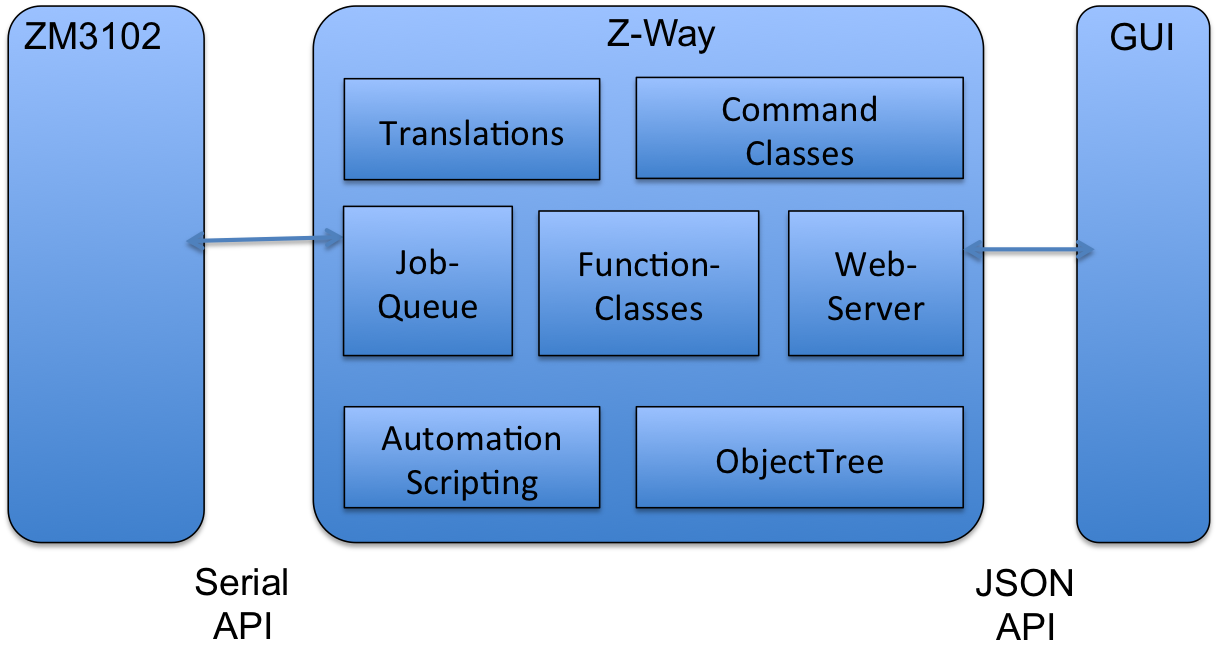
\includegraphics[scale=0.6]{pics/zway1en.png}
\caption{Z-Way Software Structure}
\label{zwaystructure} 
\end{center} 
\end{figure}

Z-Way consists of several function blocks:

\begin{itemize}
\item The Job Queue: This is the core of Z-Way
\item Function Classes: The implementation of all the commands to control the Z-Wave transceiver chip and the Z-Wave network
\item Command Classes: The application level commands used to control Z-Wave devices in the network
\item The JSON web server: It implements the application programmers interface
\item Translation Functions: They help to translate machine readable tokens into human-readable strings
\item The automation and scripting engine: This is the way to get the intelligence into the system.
\end{itemize}

\section{How to use Z-Way}


\begin{figure} 
\begin{center}
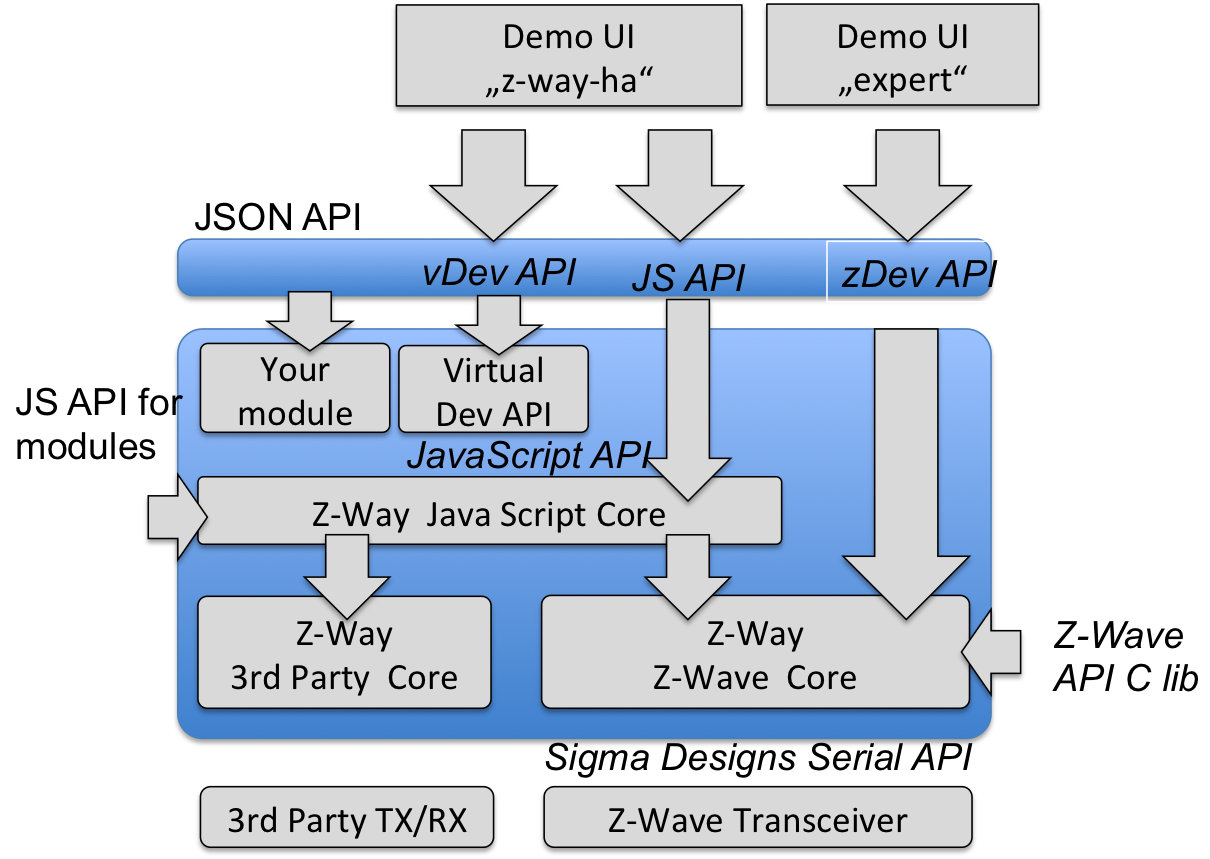
\includegraphics[scale=0.6]{pics/apis.png}
\caption{Z-Way APIs and their use by GUI demos}
\label{apis} 
\end{center} 
\end{figure}

Z-Way offers multiple Application programmers interfaces thats are partly built on each other.
Figure \ref{apis} shows the general structure with focus on the APIs. The most important part of
Z-Way is the Z-Wave core as introduced on the previous section. The Z-Wave core uses the standrad
Sigma Designs Serial API ot communicate with a Z_Wave compatible transceiver hardware. This
interface is not public but available only for owners of the Sigma Designs Development Kit (SDK) 
\footnote{The Sigma Designs SDK is available from Digikey (www.digikey.com). Depending on the 
hardware options chosen the price varies between 2000 and 4000 USD}.

The Z-Wave Core offers can be accessed directly using the Z-Wave Device API. There are two
Z-Wave Device API version available:
\begin{itemize}
\item JSON REST API: All functions are available using a JSON REST API implemented by an 
embedded webserver. The "Expert" UI is using this interface and serves both as programmers 
UI to operate the network and as reference implementation to demonstrate the use of this 
API. The Expert UI is completely written in AJAX Technology.
\item C Library API: All functions of the JSON REST API are available as C Library 
function too. In the folder /z-way-devel there are all header files with the function 
prototypes. All function calls and the whole data model are identical. The URL

http://razberry.zwave.me/fileadmin/z-way-test.zip
 
provides a sample application written in standard C that makes use of the C level API to 
demonstrate its use. Makefiles and project files for compilation on Linux and OSX are provided
with the sample application.

\end{itemize}

The Z-Wave device API only allows the management of the Z-Wave network and the control
and management of the devices as such. No higher order logic except the so called associations
between two Z-Wave devices can be used here.

For all automation and higher order logic a Java script automation engine is available.
This engine allows to write so called modules that implement a broad variety of applications
using the underlying Z-Wave devices. the automation logic can also access and use other 
third party technology stacks such as Enocean.

The Z-Way solution offers multiple prefabricated modules. One of them implements
a virtual device API. The virtual API unifies all information and control options
of the Z-Wave Device API, other third party API and own created virtual devices.
The Demo GUI z-way-ha uses this API and demonstrate the use of the virtual device API.


 
 
 

Z-Way comes with several user interfaces among them the Demo UI. The Demo UI is written in AJAX Technology 
and exposes all functions of Z-Way and the Z-Wave network controlled. This Demo UI will typically be the 
starting point for new users. The description of this Demo User Interface is not scope of this manual. Please refer to
the Z-Way Users Manual for more information.

Before a device can be used, the device needs to be included in the Z-Wave network managed by Z-Way.
This management function  is accessible in the Demo UI under the Tab 'Network'. Its one of the functions to manage the 
network. The chapter 'Function Classes' explains the different management functions and how they can be used and will
use the Demo UI dialogs as application example. The Chapter "Function Class Reference" documents all function
classes available.

The control of devices  is implemented in Command Classes. The chapter 'Command Class Implementation' is again using 
certain dialogs of the Demo UI to explain how to access these functions. (The chapter Command Class Reference 
documents all command class functions). 


In order to access device and network related data in Z-Way, knowledge of the Z-Way data model is essential.
The chapter "The Z-Way Data Model" gives the necessary insight into the data model. All data of Z-Way
are exposed on the Demo UI.

There are three ways to access and work with Z-Way. All three Application Programmers Interfaces use the very same
function and command classes and the same data model but differ in their syntax and the way they access data.



\section{API Overview}

All communication between the User Interfaces and Z-Way is handled using a 
web-technology-based  JSON Interface provided by a built in web server.

There are different Application Programmers Interfaces available for Z-WAY that serve 
different purposes:
\begin{enumerate}
\item Z-Wave Device API
\item Third Party Technology APIs
\item Virtual Device API/Business Logic API
\end{enumerate}

\subsection{Z-Wave API Overview}

The Z-Wave API is the raw access to the Z-Wave network. It shows the Z-Wave devices in 
their physical configuration and the command classes implemented.  Multiple instances of 
a device (similar functions on a physical device addressed using the Multi Channel 
function of Z-Wave) and different device functions implemented on a certain device are 
accessed using this very device.

Z-Wave network management functions are also available on the Z-Wave Device API only.

The Z-Wave Device API can be accessed using the path 

http://YOURIP:YOURPORT/ZWaveAPI/*

Device objects are accessed by 

ZWaveAPI/devices[*].* the whole data tree of the Z-Wave network is accessed using  ZWaveAPI/Data/*

\textbf{Attention: The Installer UI is a complete reference of the Z-Wave API. It shows how 
to use all function, it reveals the dynamics of the stack backend and visualizes all 
internal variables accessible on the API. The Installer UI can be accessed using the 
URL $http://YOURIP:YOURPORT/installer$}

\subsection{Third Party Technology API}

Third party Technology APIs implement the same logic as the Z-Wave device API for other 
wireless technologies such as Enocean.

For more information  please refer to the technlogy specific descriptions.

\subsection{Virtual Device API}

The Virtual Device API is an abstraction on top of (1) and (2). All physical devices 
are mapped to virtual devices but functions and channels are separated . In case the 
Z-Wave API shows one single physical device with two channel he virtual deivce API will 
show two devices with one function. In case the Z-Wave API shows a physical device with 
several different functions (like a binary switch and a analog sensor in one device) the 
virtual Dervice API will show them as several devices with one function each.

The Virtual Device API also offers access to automation logic implemented as modules.
Modules are plug ins writtenin Javascript, that access virtual devices and may create 
additional virtual devices with combined  or enhanced functionality based on certain logic.

The virtual device API is optimized for usage on a GUI. Every virtual device (with one 
single function, either as one single physical device or a part of a physcial device or 
creates by a module script) is represented by a widget. 

These widgets can be shown in a GUI. Different properties such as location of other 
tags can be assigned ot these virtual devices.

The virtual devices API also implements events and notifications usable in a Graphical 
User Interface.

Virtual devices can be access using the path http://IP:PORT/ZAutomation/

\textbf{Attention: The Home Automation UI is a complete reference of the Virtual Device API. 
It shows how  to use all function and visualizes all  backend variables accessible on the API.
The Home Automation UI can be accessed using the URL http://YOURIP:YOURPORT/z-way-ha
}

\subsection{Comparison}

The two APIs (Z-Wave) Device API\footnote{The statements are equally true for any third
 party wireless technology API} and Virtual Device API serve different purposes:

\begin{itemize}
\item The device API represents the (Z-Wave) Devices as they physically are, the virtual 
device API offers a device abstraction that represent specific functions of physical devices 
only
\item All available functions of a device are accessible using the (Z-Wave) Device API. 
The virtual device API only offers those functions that fit int oa unified device model 
usable by both physical and virtual devices.
\item The (Z-Wave) Device API allows managing the Z-Wave network, the virtual device API 
does not.
\item The virtual device API allows accessing automation functions, the Z-Wave Device API 
does not
\item Its recommended to use the Virtual Device API for device and function related
UIs of a Smart Home System but the Z-Wave Device API for the control and the management 
of the network.
\item It is possible to mix both APIs.
\end{itemize}





 